% chapter1.tex (Chapter 1 of the thesis)

\renewcommand*{\thefootnote}{\arabic{footnote}}
\setcounter{footnote}{0}
\section{Goals}

In this section, I examine the interfaces used to communicate music, and synthesise a working model of ways to notate techniques that can interface with traditional Western musical notation, and extend it.
The argument being put forth is that much like a language, music notation evolves naturally, with new `words' being developed when no suitable existing `word' is found.
The system which I propose is not a constructed language like Lojban or Esperanto, which take an opinionated and prescriptive approach to language. 
Rather, the method is more like compiling a list of morphemes encountered in existing works, breaking down our existing musical language into its elements so that compoundment, affixation, and other methods of constructing new `words' may occur naturally.
With this system, we will be able to establish a dictionary of existing symbols, as well as their function.
Composers that seek to notate in new and different manners will be able to take the symbols and interfaces a la carte, and construct their own, specific to their needs.
In instances of entirely novel concepts, this morphemic catalogue can be applied using mimetic principles to communicate intent clearly.

\section{Literature Review}

\subsection{Overview of Semiotics}

A brief overview of semiotics is necessary in order to contextualise the intent and methodology that is used.
Semiotics, the study of signs (read: meaningful communication), was invented concurrently by Ferdinand de Saussure and Charles Sanders Peirce independent of one another.\fxnote[]{saussure}
The most appreciable difference between their models was that while Saussure held that signs were made up of a signifier (the form of the sign) and signified (its meaning), Pierce's model also had an interpretant; the object that the audience interprets the signified as (since it is impossible to replicate meaning perfectly).\fxnote[]{pierce}
Signifiers are then broken up into three discrete categories; 
\begin{itemize}
\item \emph{\gls{icon}}: which have a direct physical connection to the signified. Photographs are an example of icons.
\item \emph{\gls{index}}: which show evidence of the signified. The most common example being smoke indexing fire.
\item \emph{\gls{symbol}}: which have no resemblance between the signifier and the signified; their meaning must be culturally learned. Arabic numerals, the radioactive symbol, and flags are all symbols.
\end{itemize}

Finally, our signs have two channels of information.
\begin{itemize}
\item \emph{\gls{denotation}}: the basic or literal meaning of the sign (i.e.\ a picture of a rose signifies the flower of the genus \emph{Rosa} of the family \emph{Rosaceae})
\item \emph{\gls{connotation}}: the secondary, culturally inferred meaning; a rose might also signify passion or love, depending on the context.
\end{itemize}

Interpreting these signs is described as semiosis, which Philip Tagg states is `simply the process by which meaning is produced and understood.'\autocite[156]{taggMusicMeaningsModern2013}
Semiosis happens constantly; the process of converting these words into the understanding of the concept of semiosis is, in itself, semiosis. 
Pierce argues that in between the audience and the signifier, during the process of semiosis there is the interpretant, an object that the audience creates that represents the signified (because a dog cannot exist inside our heads, but merely the idea of a dog; the reality of the dog will never be fully realised inside the mind because it lacks the gestalt of the physical thing; 
it's a construct, unable to approach the truth of the dog by virtue of its limitations).\fxnote[]{pierce}
Semiosis is an important step, as the interpretant which Peirce describes is unique to the audience; we construct meaning completely independently, informed by our past experiences and knowledge.\fxnote{citation needed Pierce}
Thus, the same picture of an aunt's dog may be interpreted by the aunt as being a loving pet, whereas a neighbour might interpret the image more negatively, as `the annoying dog that wakes me up at 6am'.

Looking at Western notation, we have several instances where a symbol may hold a different context depending on the interpreter's experience-- 
the same notation is used for a harmonic and a note that is meant to be played open on a French horn.\autocite[]{schuilingNotationCulturesEthnomusicology2019}
If a musician was given a piece of sheet music without any indicator of the instrument that it was written for, their experience (or lack thereof) with one of the instruments may influence how they choose to interpret the symbol.
John Fiske categorises \begin{quotation}
    denotation [as] what is photographed, connotation [as] how it is photographed
\end{quotation}.\autocite[91]{fiskeIntroductionCommunicationStudies2011}
What the composer chooses to put on the page could be argued to be denotative, while what is omitted and how the material is presented is connotative.

Semiotics is particularly applicable in web design, where intuitive `notation' is sought after to reduce the `friction', or difficulty a user has navigating a site.
We can learn many things from the research that has been done into how to use skeuomorphic design to convey an element's function.
Our goal with constructing intuitive music notation is to reduce the `friction' just like a web designer, using design patterns that are intuitive even to people that are unfamiliar with the content.
We can use the connotations of existing symbols to help infer how we can construct new symbols.
As an example, the line that makes up a glissandi can be either straight, or wavy, as seen in \autoref{fig:Glissando}.
\begin{figure}
    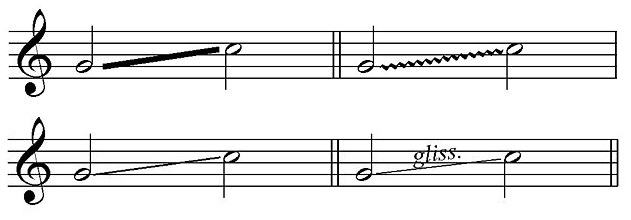
\includegraphics[]{./resources/glissando.jpg}
\caption{Various styles of glissandi}\label{fig:Glissando}
\end{figure}
The similarity of the last two examples on the right to the notation for \emph{portamento} results in a connotation with those two types being continuous, rather than having discrete pitches.
Additionally, the interpretant's instrument may also influence the meaning to them- timpanists and trombonists are more likely to interpret glissandi as continuous changes, while pianists interpret step-wise due to the nature of their instruments.\fxnote{need to find a citation for this}
In this way, we understand that the meaning of a symbol is tied inextricably with the culture of the interpretant; attempting to make use of this cookbook for an audience not `primed' to understand it (i.e.\ one unfamiliar with Western art music conventions) is doomed to failure.
In order to produce a document that can be used reliably, the work must either be totally objective (a fool's errand in the pursuit of extracting cultural understanding of signs), or cognisant of the pitfalls and assumptions made.
To this end, the `cookbook' necessitates disclaimers specifying the assumptions made; terminology or notation used specifically in avant-garde or Renaissance music will not have any transitive qualities aiding its uptake to an audience that is not familiar with the source material.

Some symbols are not compatible with one another; a properly engraved work will never have an upbow and downbow on the same note, as the two symbols fulfill the same function (unless, of course, the two symbols are joined together, which denotes a rapid rebowing).
This is what is known as a paradigmatic relationship; by virtue of the presence of one, it excludes the possibility of the other.
Looking at web design, we can draw a somewhat rough parallel to drop-down menus; there's only one slot that can be filled.
Other examples of paradigms would be the degree at which a French horn opens or mutes their instrument, which is not a binary, but a scale of `openness'.

Understanding the properties of a sign that are inherited from its history, context, and role informs what information is necessary to communicate to the reader in order for them to be able to make use of the `cookbook'.
Without a cohesive and holistic (or rather, as holistic as is possible) treatment of the signs, the intent of the `cookbook' falls short; composers must be armed with the knowledge of the context in which the sign developed, and its use in order to be able to make informed decisions.



\subsection{Argument}
% The perhaps hyperbolically described `cult of the written score' in the 20th century New Complexicist movement saw the rise of composers prescribing more and more parameters.
In the 20th century, the `cult of the written score' developed, in which the composer prescribed more and more parameters to be interpreted literally.\fxnote{citation very much needed}
This was in part fueled by contemporary composers being strongly opinionated in how their works should be interpreted, and partly because of the styles-- the sheer breadth of the number of parameters specified in New Complexicist works makes the interpreter pre-biased to assume that there is little room for interpretation.
This has permeated through to an underlying culture of assuming that when performing a work by a living composer that, if they wished for it to be interpreted a specific way, they would have specified that.\fxnote[]{can't really cite this}
There have been several notable theses on the philosophy and reasons behind the New Complexicist movement, and it would be ill-advised to retread tired arguments.
All that is relevant to this study is that it can be argued that ultimately, music notation is an imperfect representation of the perfect, Platonic ideal, which exists only in the mind of the composer. 
This is to say that notation is the physical manifestation of a perfect ideal, an interpretant which exists only in the composer's mind, imperfectly represented in the physical form.

Floris Schuiling describes music notations as \begin{quotation}
`interfaces for imagining virtual musical relations'
\end{quotation}
which is an apt description; similar meaning can be derived from verbal instructions, and the notation used is merely a vehicle through which to deliver the instructions on how to play the work.
The end result of this is that the precise vehicle through which performers obtain their instructions can be modified, mutated, and otherwise changed to better represent the imagined musical relations as the composer envisages.
This is done often when the traditional structure of Western music notation fails to account for some niche that it was not designed for; the aleatoric works of John Cage, stochastic aleatoricism of Lutoslawski, and many others who sought to extend the artform to its metaphorical breaking point.
Their modifications and adaptations of notation have, to varying degrees, taken root, and become accepted into the canon as valid notation; it is unlikely that the reader would have any doubt of the intended effect if presented with a Bartok pizzicato symbol above a string instrument's note.
However, these notations have been developed independent of one another, and in the current musical sphere, we are faced with an ever-increasing list of symbols to memorise, along with lengthy descriptions littering the frontmatter.
Every composer that creates new notation (be it the notation of a technique, a method of notation, or an entire interface) is effectively treading new ground.
On occasion, multiple notations are created for the same technique, such as the multitude of ways that composers communicate \fxnote{TODO find example technique with duplication}.
However, duplication of technique is not necessarily a bad thing; `hairpin' crescendos and textual instructions both serve largely the same function.
In other cases, such as the notation for \fxnote{TODO find a better example than subharmonics} subharmonics, notations differ in specificity. 
Crumb's notation method has the least specificity, denoting simply a `scratchy tone' \fxnote{TODO find Crumb's quote}, while Kaija Saariaho specifies the relative degree of pressure to apply.
Mari Kimura's method specifies the resultant pitch, but omits the relative pressure required to obtain the tone.
These methods of notation are all for the same technique, but focus on different aspects, according to what is desired by the composer.
It is this philosophy that this thesis intends to address; 
providing a toolbox of components that a composer can use to construct new notation, as well as cataloguing existing notations so that composers may better communicate their intent, to make the interface that they create closer resemble the interpretant that exists in their head.

Of particular interest is the work of Ellen Fallowfield, whose thesis, `CelloMap' website and recently, application, form a comprehensive and holistic review of the ways in which a performer may `map' actions onto a cello.\autocite[]{fallowfieldCelloMapHandbook2009,fallowfieldCelloMap}
This non-opinionated and genericized method of cataloguing actions sees its contents applicable where a more specific approach would fall short, ensuring that it does not fall out of date.
In a similar way, I aim to catalogue actions from a composer's perspective, providing a suite of tools with which a composer can construct a notation to suit any imagined circumstance; be it using an animated score that changes with time, a score seen within a VR headset, or any other interface that may develop in the future.

There has been much research done into the ways that computers can interpret sheet music, an extension of OCR technology which has resulted in several market-ready tools such as PhotoScore. 
More pursuant to this study are the developments of machine-readable formats such as the GUIDO music notation system, if only as examples of the parameters that must be accounted for.
The thesis `denm' makes a comprehensive study of many of the strategies and reasons that performers will mark up a score with annotations. 
Additionally, it goes into discussion of the various accessibility and printing issues associated with using CYMK colour in printed scores.\autocite[22--29]{beanDenmDynamicEnvironmental}
denm (Dynamic Environmental Notation of Music) is a 

Kurt Stone identifies many of the issues present in modern notation in his 1963 article in \emph{Perspectives of New Music}, and he states that \begin{quotation}
    `no other aspect of contemporary notation is more desperately in need of fundamental revision than that of rhythm.'
\end{quotation}, arguing that the existing systems of notating rhythmic ideas are either insufficient, poorly tooled, difficult to implement, or otherwise not suitable for purpose.\autocite[20--22]{stoneProblemsMethodsNotation1963}
Stone explores proportional notation as used in Stockhausen's \emph{Zeitmasse} and Cage's \emph{Music of Changes} (1951), identifying an issue where accidentals can interfere with precise placement of notes. 
This proportional notation system is very similar to the piano roll, or \emph{pianola} that is found in many Digital Audio Workstation workflows, such as Ableton, FL Studios, and Pro Tools.
The piano roll notation is arguably a superior method, as it is as literal as can be, assigning pitch to the y axis (with the label of the y axis being the matching piano key), and time to the x axis, often representing the metrical grid with lines.
However, while this workflow is suitable for DAWs, it is cumbersome to use in performance settings, and cannot be considered a genuine alternative for mapping music to an interface for performance purposes.
Stone notes this, recognising how proportional notation is ill-fitted to performer parts due to rhythmic explicitation via a `middleman' of a commonly agreed metrical unit being replaced with the much more subjective relational measurement; a crotchet is explicitly a crotchet, but a 3.3cm distance may be approximated to an imprecise element.
This can be mitigated with a common `cue' stave in parts, but as size of the ensemble grows, practicality decreases.

Stone describes notation as \begin{quotation}
    [\dots] a system of directional signs which [is] used to enable a performer conversant with them and and with the musical conventions of the era during which they were in use, to recreate a composer's \emph{artistic} vision on the basis of what the \emph{mechanical} directions implied.
\end{quotation}

He continues, stating that \begin{quotation}
    [some] of today's music is constructed in such a way that the slightest modification of \emph{any} of its measurable elements is likely to distort the inner logic of the entire work.
    In such music, only rigid sign realization is admissable; this music does not permit ``interpretation''. 
    At the same time, however, music of this nature is generally so complex that truly accurate sign realization is rarely if ever achieved in performance.
    Thus, the score and the performer have actually exchanged roles: whereas the score used to be the map designed to guide the performer towards the composer's artistic vision, it now is often completely explicit.
    On the other hand, performances are now often mere stabs in the direction of the composer's envisioned perfection of execution.
    The imprecision and variability of human performance are actually quite detrimental to the requirements of totally organized and predetermined works.\autocite[30--31]{stoneProblemsMethodsNotation1963}
\end{quotation}

This broad criticism of the failings of New Complexicists touches at the core of the issue; an imperfect relational system will produce imperfect results.

In the paper `Animated Notation, Score Distribution and AR-VR Environments for Spectral Mimetic Transfer in Music Composition', which deals with applying graphic scores to a new, Virtual Reality context, Jonathan Bell and Benedict Carey note that \begin{quotation}
    `the closer a musical unit gets to representing a direct action (that is, the movement of an object in space) the more mimetic it becomes.'\autocite[]{bellANIMATEDNOTATIONSCORE2019}
\end{quotation} This observation is paralleled with the 

While the generation of new methods of presenting music past the simple paper score is not a focus of this study, there is still much to be learned from the research that has been carried out in these fields.
Animated scores, as pioneered by Cat Hope and others are a relatively straightforward development of the static score as it exists in printed form, augmented with features such as playback lines, and dynamic elements.
`Inventing Malleable Scores: From Paper to Screen Based Scores', a paper by Arthur Clay introduces the concept of malleability to score creation and interpretation.

This thesis aims to provide the composer with more tools to aid in the specificity of the work, so that they may more accurately and concisely communicate the desired techniques.

This PhD continues upon the previous research that I conducted during my Honours, and there is significant overlap with the two topics.
Therefore, the first item that is worthy of mention would be `Harmonic Based Extended Techniques and their Compositional Applications', which includes a ground-level review of the seminal literature in the field.\autocite{grayHarmonicBasedExtended2019}
However, due to the limited scope of the exegesis, there were significant omissions, so for the sake of completeness its contents will be reviewed under the lens of `composing with extended techniques'.
Additionally, there are a number of sources that were either missed or cut from the initial literature review for sake of brevity.
% There appears to be a great deal of activity in similar spheres of research in Basel, Switzerland, and there are several manuscripts and texts that appear only in German.

Unlike standard pedagogical models, wherein the student learns from the teacher, the methods used in this exegesis are a more collaborative, and less rigid practice.
Composers typically will have a performer in mind when they compose a work, and collaborate with them, working to find what works for the artists and instrument.
However, in subsequent performances, that direct connection to the composer is often unavailable, and the performer is left to interpret the paratext, without direct instruction from the composer.
Paratextual instruction can vary in degrees of specificity, and will often be printed in the frontmatter of the work.
Where there is a well established understanding of the technique (such as the Bartok pizzicato technique, which has been accepted into the canon of `standard' techniques, and is no longer considered extended), this is not an issue, but can pose issues in the case of techniques where there is a great deal of variance possible, such as multiphonics and subharmonics.
In some cases, the performer must rely on previous works to build a contextual language in which to interpret esoteric markings, or use previous recordings of interviews and performances to ascertain the composer's intent.
Understanding the composer's intent is a crucial part in the preparation process, and the ability to accurately reproduce the composer's intent may negatively impact a work's longevity in the literature.
Many academics have recognised the deficit in training in extended techniques, both in their base form and their composer-specific implementation (which may vary from composer to composer, or piece to piece). 
Violist Sarah Wei-Yan Kwok discusses this in her thesis `Breaking the sound barriers: extended techniques and new timbres for the developing violist', where she commissions six etudes for viola exploring extended techniques, along with an investigation into pedagogy.\autocite{kwokBreakingSoundBarriers2018}

The composer-performer collaboration dynamic has been explored at length; the most famous example being the virtuoso pianist Paul Wittgenstein, whose career came to a halt during World War 1, when he lost his right arm.
Afterwards, he began commissioning leading composers to write for him, resulting in Richard Strauss', `Parergon zur `, `Sinfonia Domestica for Piano and Orchestra', Maurice Ravel's `Piano Concerto for the Left Hand in D major', and further works written by Hindemith, Korngold, Britten, and Prokofiev, to name a few.\autocite[107]{predotaPaulWittgensteinVoice2014}
Collaboration with the intended performer is crucial to a composer's ideas being realised accurately, as articulated by Jack Barnes, who stated:
\begin{quotation}
    My collaboration with Mathieson-Sandars allowed for subtle but important improvements to \emph{Lines, Contexts and Freedoms}. 
    Certain aspects such as the composer hearing his piece for the first time, experimenting with different pianistic timbres and creating more comfortable hand distributions were among the most useful outcomes of our collaboration. 
    As the performer, it was useful for my interpretation to learn [the composer's] intent behind the gestures; that the effect of dynamic shaping was not desirable for all of them.\autocite[20]{jackbarnesExaminationComposerPerformerCollaborations2017}
\end{quotation}
Discussion being needed with the composer to learn the composer's intent suggests that there was information being provided to Barnes that was not present in the paratext.
Future performers of the work that was commissioned by Barnes may not have the same level of access to the composer, hence the need for a thorough and precise documentation of the intended sound being available.

Sheet music is an abstracted conception of a musical work; the printed paper is merely a set of instructions that are interpreted by the performer, in order to express a musical idea that only the composer truly knows.
Without a perfect abstraction of what the composer imagines, a `perfect' reproduction is impossible.
Indeed, even if there \emph{was} a perfect reproduction, the variance in instrumental timbre and other facets of the process render it a fool's errand.
The Platonic ideal is unattainable, and perhaps why little effort has been made to make further progress towards the liminal.\fxnote{citation needed, obviously}

Attempts at combining notation with composer intent have been made, with Eftiha Victoria Arkoudis' `Contemporary Music Notation for the Flute: A Unified Guide to Notational Symbols for Composers and Performers' building on the work of Robert Dick.\autocite{arkoudisContemporaryMusicNotation2019}

Instructive manuals are typically in one of two categories; performer-oriented, in which the techniques presented are articulated in a performer-focused context, and composer-oriented; orchestration manuals which dictate the end results.
For brevity, these usually do not intersect, or at least are not written comprehensively with both the composer and performer in mind. 
The lack of literature that encompasses the entirety of the production of sound process, from the action to the resultant, is slowly being rectified, particularly with online resources such as Heather Roche's work in clarinet multiphonics, and Fallowfield's with CelloMap gaining popularity.\autocite{rocheHeatherRoche, fallowfieldCelloMap}
\subsubsection{Notation Manuals}
Notation has long been the domain of Kurt Stone and Gardner Read being the authoritative voices, writing extensively on the subject beginning in the 1970s.\autocite{stoneMusicNotationTwentieth1980,readCompendiumModernInstrumental1993,readContemporaryInstrumentalTechniques1976,readMusicNotationManual1979a}
Additional texts by David Cope and Erhard Karkoschka supported these with their own contributions.\autocite{copeNewMusicNotation1976,karkoschkaNotationNewMusic1972}
Editor of Faber Music, Elaine Gould's seminal `Behind Bars' gave an authorative voice to the methods of notating along with the building blocks for techniques which she felt had not been developed to the point of consensus.\autocite[iii]{gouldBars2011}

\subsection{Physics}
In order to be able to accurately prescribe instructions on how to produce these techniques, there must be an understanding of the underlying physics.
Helmholtz provides our basic undestanding of the stick---slip motion which makes a bow produce sound on a string.\autocite{helmholtzSensationsTonePhysiological1954}
Knut Guettler and Håkon Thelin have provided extensive research into how the string can produce multiphonics.\autocite{thelinAnalysisBowedStringMultiphonics,thelinMultiphonicsDoubleBass2011,guettlerBowedstringMultiphonicsAnalyzed2012,guettlerGuideAdvancedModern1992,guettlerWaveAnalysisString1994}
\fxnote{This needs to be expanded}{R. T. Schumacher, Kenneth Marskall, and Anders Askenfelt contribute additional aspects to the literature.}\autocite{schumacherTransientBehaviourModels1995,askenfeltMeasurementBowingParameters1989,marshallModalAnalysisViolin1985}
For subharmonics, the violinist that discovered the technique, Mari Kimura, has contributed practical examples on how to produce them.\autocite{kimuraHowProduceSubharmonics1999}
\fxnote{Empirical data on what? Expand!}{However, for research into the technique's production, Robert Mores, Guettler, Erwin Schoonderwalt, Carleen Hutchins, and John Cantrell provide empirical data.}\autocite{moresFurtherEmpiricalData2019,guettlerBowedStringDevelopment2002,schoonderwaldtViolinistSoundPalette2009,hutchinsSubharmonicsPlateTap1960,cantrellSubharmonicGenerationChaos2015}

\subsection{Extended Techniques}
To understand extended techniques, we must first establish a basis of what is considered a `regular' technique, or rather, what the qualifying factors are for a technique to be considered extended.
To do this, we will look at what techniques are commonplace in the literature, and which are less so.
Techniques that require descriptions in the frontmatter or otherwise `extend' the instrument beyond the normal canon would reasonably be understood to be considered extended techniques.
Read discusses this, stating:
\begin{quotation}
    Many so-called ‘new’ instrumental devices have developed from well established techniques; they are extensions of, or refinements of, procedures long considered part of a composer’s repertorium of expressive devices. 
    The newness, then, is not one of kind but of degree, a further and more extensive development of basic effects found in scores from the late nineteenth century to the present day.\autocite[3]{readContemporaryInstrumentalTechniques1976}
\end{quotation}
Unpacking the language that we use, extended techniques are just that; an extension of the traditional techniques that are already established in the canon. 

% \fxnote{This probably needs retooling to fit better in the literature review.}There are three aspects that are relevant to the literature review; literature surrounding the techniques themselves, literature with how the techniques are presented, and scores. 
Scores are necessary to understand how composers implement extended techniques in practice.
By reviewing their frontmatter and the symbol notation, we gain an understanding of how composers present information to performers, and can build a system of notation that maps consistently with the rest of the established canon.
Consequently, seminal scores will be included in the literature review so that we may understand how they work. 
These scores' notation systems for extended techniques will be broken down into their elements, and through comparative analysis of how different composers implement the same techniques, we will be able to find how textual, symbolic, and graphic notation systems can be used to achieve the desired results.

Dimpker postulates the following criteria for extended technique notation; \begin{quote}
    `(1.) As exact as possible and (2.) As simple as possible while the system may (3.) Not be contradictory to
traditional notation, but should instead extend and be closely related to it.'\autocite[3]{dimpkerExtendedNotationDepiction2012}
\end{quote}
This meshes well with the philosophy of Elaine Gould's `Behind Bars', which advocates for a consistent style language, despite the two texts occasionally coming at odds with one another in the exact treatment of some cases.\autocite[120--121, 61]{dimpkerExtendedNotationDepiction2012,gouldBars2011}
Dimpker posits that four methods of notation are acceptable in order to realise exact and precise notation; `action notation, symbolic notation, diagrammatic notation, and schematic notation'.\autocite[33]{dimpkerExtendedNotationDepiction2012}

Textual notation, i.e.\ instructions printed in the score, are the most straight forward, but limited to what can be summarised in few words.
Symbolic notation assigns the technique to a symbol, typically with the instructions placed in the frontmatter.
Graphical notation systems are often used when the binary of symbolic notation is restrictive, and requires a greater fidelity than textual notation can provide. 
An example of this can be seen in Kaija Saariaho's notation of overpressure, wherein she uses a black bar to represent the amount of overpressure required, temporally relational to the position in the score.\fxnote{TODO:saariaho citation}

\subsubsection{Double Touch Harmonics}
The technique of `double touch harmonics' as described by John Addison appears to be almost totally novel. 
Chase T Jordan references the technique briefly as `dual node harmonics', but provides only a basic overview of their treatment.\autocite[36]{jordanOldInstrumentsNew2020}
The only other reference that seems to be relevant is a 1980 thesis, which has not been made available online.\autocite{woodrichMultinodalPerformanceTechnique1980}
Addison has completed several fingering charts and made preliminary instructive documentation on the technique, which has been provided to the researched.
Due to the lack of literature, collaboration with performers will be essential in order to build the technique to a stable, usable state.

\subsubsection{Subharmonics}
No significant output in the research of the mechanics of subharmonics has occurred since the publication of my Honours exegesis, though there have been several works composed which make use of subharmonics.\

\subsubsection{Multiphonics}
Multiphonics have been well-documented in reed instruments, with Robert Dick's seminal `The Other Flute', setting the gold standard in extended technique documentation, painstakingly notating the outputs, fingerings, and qualities of flute multiphonics and other extended techniques.\autocite{dickOtherFlute1989}
There are several Barenreiter technique manuals for other aerophones that cover multiphonics, including bassoon, saxophone, violin, and oboe, with the publisher appearing to try and compile a manual for every instrument.\autocite{weissTechniquesSaxophonePlaying2010,galloisTechniquesBassoonPlaying2009,ardittyTechniquesViolinPlaying2013}
\fxnote{Double check to see if this is true}The book on violin by violinist Irvine Arditty notably lacks any information on multiphonics, perhaps due to the difficulty of production on the small instrument.\autocite{ardittyTechniquesViolinPlaying2013}

\paragraph{String instruments}
The development of literature dealing with multiphonics on stringed instruments is more recent, with a special January 2020 Tempo journal issue, dedicated entirely to string multiphonics.
It was collated by Dr.\ Ellen Fallowfield, who notably contributed the landmark thesis CelloMap (and eponymous website) in 2009.\autocite{fallowfieldCelloMapHandbook2009, fallowfieldCelloMap}
Her article, `Cello Multiphonics: Technical And Musical Parameters' expands upon the work that she began in her thesis, `CelloMap'.\autocite{fallowfieldCelloMultiphonicsTechnical2020}

\paragraph{Plucked chordophones}
Rita Torres has explored multiphonics on the guitar extensively, with several papers dedicated to their research, including her thesis, `A New Chemistry Of Sound: The Technique Of Multiphonics As A Compositional Element For Guitar And Amplified Guitar'.\autocite{torresMultiphonicsCompositionalElement2012}
Paulo Ferreira-Lopez and Torres provide a robust exploration of previous systems of notation of multiphonics, suggesting notational methods similar to those that Fallowfield suggests.\autocite{ferreira-lopesGuitarMultiphonicsNotations}
Catalogues of multiphonics in the guitar literature show that there has been little interest in the technique, with the first score dating back to 1832, but only around twenty or so pieces composed since the techniques inception.\autocite[80--82]{torresSoundWorldGuitar2018}
It has been suggested that the widespread adoption of the technique has been marred by the mode of playing naturally having a decay, making multiphonics more difficult to hear for an audience, as well as the guitar having a poor dynamic range.\autocite[21--22]{Torres2014TowardsOT}
This has been all but confirmed with the analysis of multiphonic signal decay at distances equivalent to that of an audience revealing that without amplification, the multiphonics will be inaudible.\autocite[279]{torresGuitarMultiphonicsInfluence2014}
Thomas Ciszak and Seth Josel expand upon the research carried out by Torres, collating a catalogue of performable multiphonics from strings 3 --- 1, and examining multiphonics on the electric guitar.\autocite{ciszakNeonLightMultiphonic2020}

\paragraph{Piano}
The piano, an unlikely candidate for multiphonics, has had some success in making inroads in the technique through the use of preparing the piano.
With the development of more robust literature, the prospect of developing a new sound-palette for the piano is alluring.
Interest begins in 2016 with Juhani Vessikala's MA thesis on the topic.\autocite{vesikkalaMultiphonicsGrandPiano2016}
Sanae Yoshida acknowledges Vessikala's work in an article in the multiphonics issue of Tempo, where Yoshida expands upon the practical ways in which a composer can use microtonality (and multiphonics) on a piano.\autocite{yoshidaMicrotonalPianoTunedIn2020}
Following is Caspar Walter's algorithm to calculate the frequency components of pure multiphonics.\autocite{casparjohanneswalterVariantsContinuedFraction2019}